\documentclass[12pt]{article}

\usepackage{standalone}
\usepackage{nccfoots}
\usepackage{graphicx}
\usepackage{bbold}
\usepackage{fancyvrb}
\usepackage{braket}
\usepackage{color}
\newcommand{\ops}[1]{|#1$\rangle$$\langle$#1|}
\newcommand{\opd}[2]{|#1$\rangle$$\langle$#2|}
\newcommand{\opdu}[3]{|#1$\rangle$_#2$\langle$#3|}
\newcommand{\opq}[4]{|#1 #2 $\rangle$$\langle$#3 #4|}
\definecolor{mygreen}{rgb}{0,0.5,0}
\definecolor{myblue}{rgb}{0,0,0.75}
\definecolor{mymagenta}{cmyk}{0,1,0,0.12}
\usepackage[colorlinks=true,
   linkcolor=blue,
   citecolor=blue,
   urlcolor =blue]{hyperref}

\newcommand{\btext}[1]{{\color{myblue} #1}}
%\newcomm	and{\gtext}[1]{}
\newcommand{\gtext}[1]{{\color{mygreen} #1 }}
\newcommand{\mtext}[1]{{\color{mymagenta} #1}}
%\newcommand{\citeSM}{\cite[SM][]{SM}}
%\newcommand{\citeSM}{\cite[$^\mathrm{SM}$][]{SM}}
\newcommand{\citeSM}{\cite[{\tiny SM}\kern-0.3em][]{SM}}
\newcommand{\be}{\begin{equation}}
\newcommand{\ee}{\end{equation}}
\newcommand{\rtext}[1]{{\textcolor{red}{#1}}}
\newcommand{\cf}{{\it cf.}}
\newcommand{\ie}{{\it i.e.}}
%Uncomment next line if AMS fonts required
\newcommand{\der}[2]{{\frac{d #1}{d #2}}}
\newcommand{\beq}{\begin{eqnarray}}
\newcommand{\eeq}{\end{eqnarray}}
\def\bgrk#1{\mbox{{\boldmath $#1$ \unboldmath}}\!\!}
\def\eq#1{(\ref{#1})}
\def\H1{\widehat{H}_1}
\def\M{\hbox{\large \tt M}}
\def\dmat{\hbox{\large \tt d}}
\def\G{\slash\mkern-11muG}
\def\ug{\underline{\gamma}_2}
\def\pl{\partial_{\Lambda}}


\expandafter\let\csname equation*\endcsname\relax

\expandafter\let\csname endequation*\endcsname\relax

\usepackage{amsmath}
\usepackage{amssymb}


\begin{document}

\title{Restaurant categories in Switzerland}

\author{Pierre-Olivier Guimond}

\date{\today}
\maketitle

\section{Introduction}

Switzerland is a small country, located in mainland western Europe. Despite its size, people in Switzerland have their own cultures, cuisines, and traditions, which, of course, have also inherited some influence from the neighbouring cultures. In this project, we are interested in investigating this influence, by studying the types of restaurants that can be found in Switzerland, and their distribution throughout the country. In particular, we will focus our attention on the french-speaking canton\footnote{Switzerland is divided into 26 cantons} of Vaud.

The problematic we wish to tackle can be expressed with the following question: ``How do the type, amount and diversity of restaurants depend on the location throughout the canton of Vaud?''. This question is of great interest for individuals wishing to open a restaurant, or for restaurant chain owners looking to open new units.    

\section{Data} 

\subsection{Data acquisition}

The canton of Vaud is divided into ten districts, which are each further divided into communes. First of all, the list of all communes in the canton can be found on the Wikipedia page\footnote{\url{https://fr.wikipedia.org/wiki/Communes\_du\_canton\_de\_Vaud}}, which contains useful information such as the related district, or the population and population density in the commune. Second, we will use the python package {\em geopy} in order to access the geocoordinates of each commune. 

Finally, we will use the {\em explore} query from the {\em Foursquare} database to obtain a list of restaurants located in each commune, and, importantly, the categories of these restaurants. The list of all possible categories can be found on the {\em Foursquare} webpage\footnote{\url{https://developer.foursquare.com/docs/resources/categories}}, as subcategories of the ``Food'' venue category.
Analysing these data will then allow us to study the relation between restaurant features (including the type of food served) and the features of the commune or district.

\subsection{Data cleaning}

First, the list and features for the communes was obtained as a table named \verb Communes. The data was pretty much clean as is, except for features such as population, area, and population density being represented by character strings rather than real numbers.

Second, the geolocation for each commune was obtained using the python package {\em geopy}, which searches the coordinates when provided the name of a location. The coordinates where obtained by searching sequentially for ``{\em $\langle$name of commune$\rangle$, Vaud, Switzerland}'', ``{\em $\langle$name of commune$\rangle$, Switzerland}'' and ``{\em $\langle$name of commune$\rangle$,  $\langle$name of district$\rangle$, Vaud, Switzerland}''. If no query found coordinates compatible with the canton of Vaud, the commune was dropped from the data.

Finally, for each commune location we gathered a list of nearby restaurants from the {\em Foursquare} database, and gathered all restaurants obtained in a table named \verb Restaurants. We dropped communes from {\verb Communes } which had no restaurant retrieved, as they do not pertain to our study. We also dropped from {\verb Restaurants } all duplicates obtained by querying using nearby communes, as well as all results where the category was not specific enough, viz. where the category was either ``Food'' or ``Restaurant''. Finally, we grouped similar categories: we relabelled the category ``Pizza place'' as ``Italian restaurant'', and relabelled subcategories of ``Asian restaurant'' (e.g. ``Chinese restaurant'', ``Thai restaurant'', etc.) as ``Asian restaurant''.

\subsection{Selected features}

The features in {\verb Communes } which were kept for the analysis where:
\begin{itemize}
\item Commune name
\item District name
\item Population
\item Area in km${}^2$ (checkmate americans)
\item Population density in people/km${}^2$
\end{itemize}
{\verb Communes } contains 308 rows. On the other hand, the features in {\verb Restaurants } which were kept for the analysis where:
\begin{itemize}
\item Name of the restaurant
\item Name of the corresponding commune
\item Subcategory of restaurants
\end{itemize}
{\verb Restaurants } contains 819 rows.

\section{Methodology}

\subsection{Commune properties and statistics}

We first discuss the properties and statistics of the communes. In Fig.~\ref{fig1}(a,b) we show the distribution of communes as a function of their population and their population density. Strikingly, most communes have a very small population, with a mean of 2590 and a median of 853.5 people. The population density is also typically very small, with a mean of 440 people/km${}^2$ and a median of 134 people/km${}^2$. On the other hand, Fig.~\ref{fig1}(c,d) represent the the distribution of people residing in communes, as a function of the population and the population density of the communes. The average person lives in a commune with 31878 people and population density of 1919 people/km${}^2$.

\begin{figure}
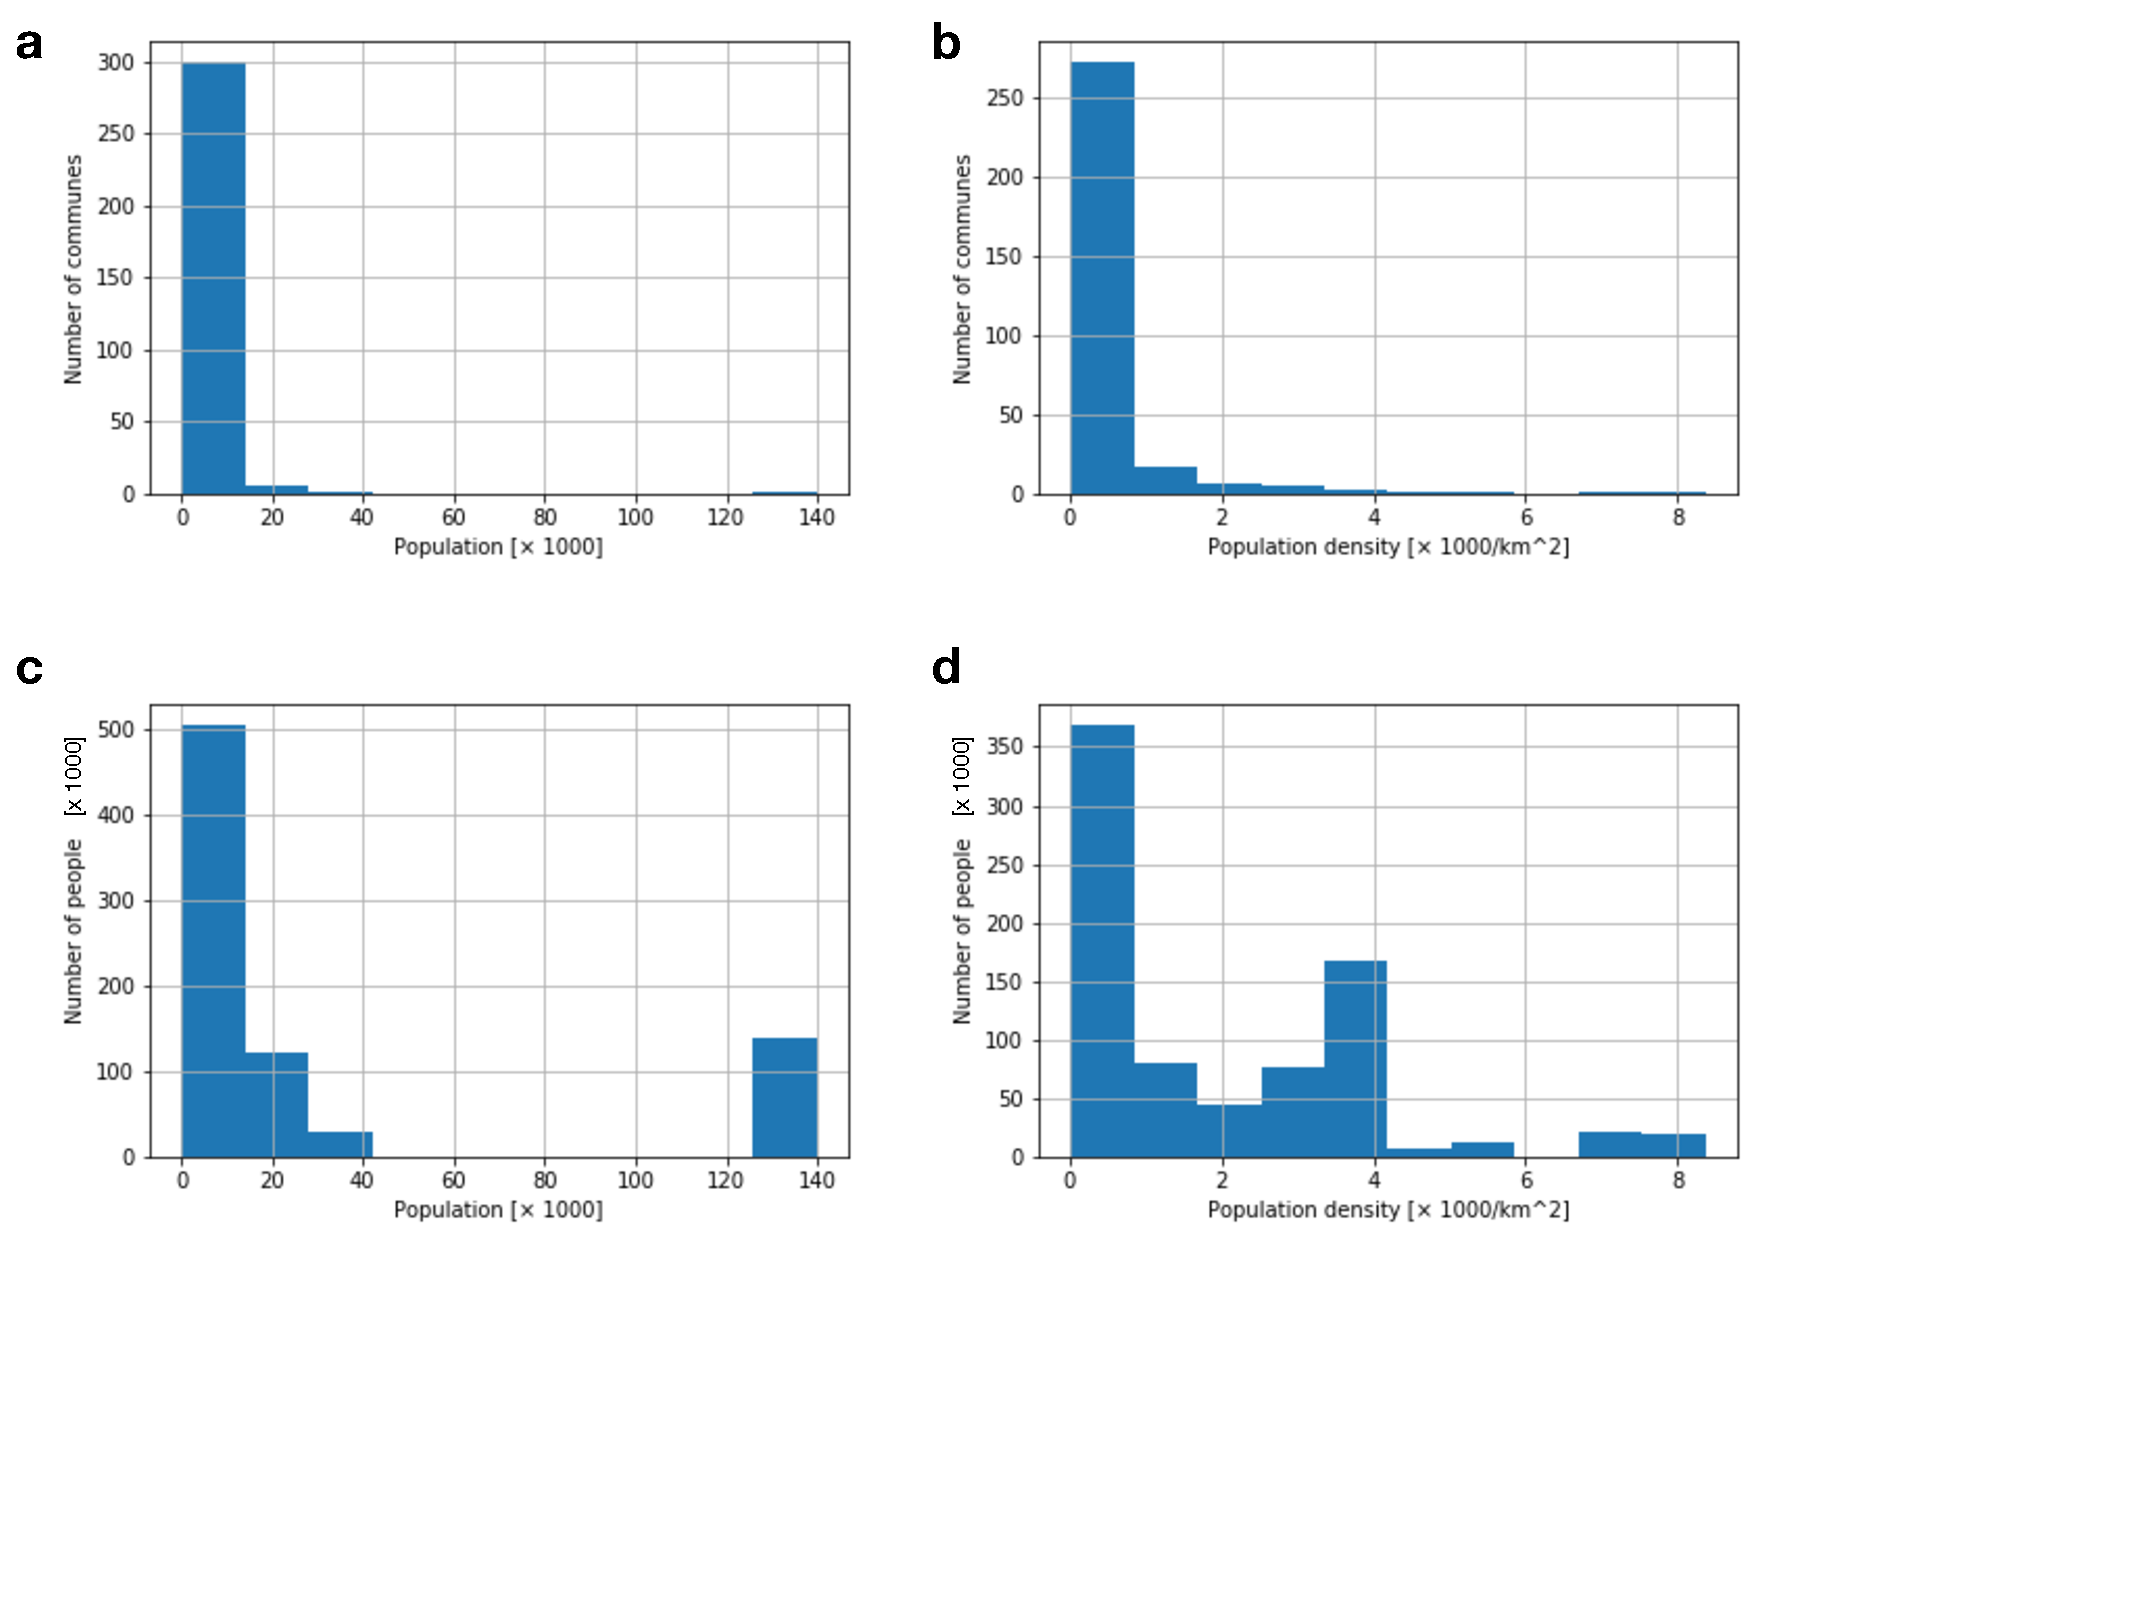
\includegraphics[width=\textwidth]{Figures/Fig1}
\caption{\label{fig1}{\em Commune properties. ---} Histograms of (a,b) communes, and (c,d) people leaving in communes, as a function of (a,c) the population, and (b,d) the population density. }
\end{figure}

In Fig.~\ref{fig2} we show the total number of restaurants obtained for each commune. The linear fit has a slope coefficient of $0.59$ restaurants/1000 people, and an intercept of $1.10$ restaurants, and we obtain for the regression an $R^2$-score of 0.89.

\begin{figure}
\begin{center}
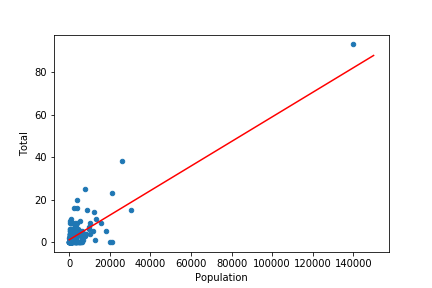
\includegraphics[width=0.7\textwidth]{Figures/Fig2}
\caption{\label{fig2} Total number of restaurants obtained for each commune, vs its population.  Red line: linear fit (see text).}
\end{center}
\end{figure}

In Fig.~\ref{fig3} we show a map of the canton of Vaud, where each commune is represented as a blue dot, with the dot radius representing the total number of restaurants. Clearly, larger dots correspond to the larger cities, which are located along the L\'eman lake. 

\begin{figure}
\begin{center}
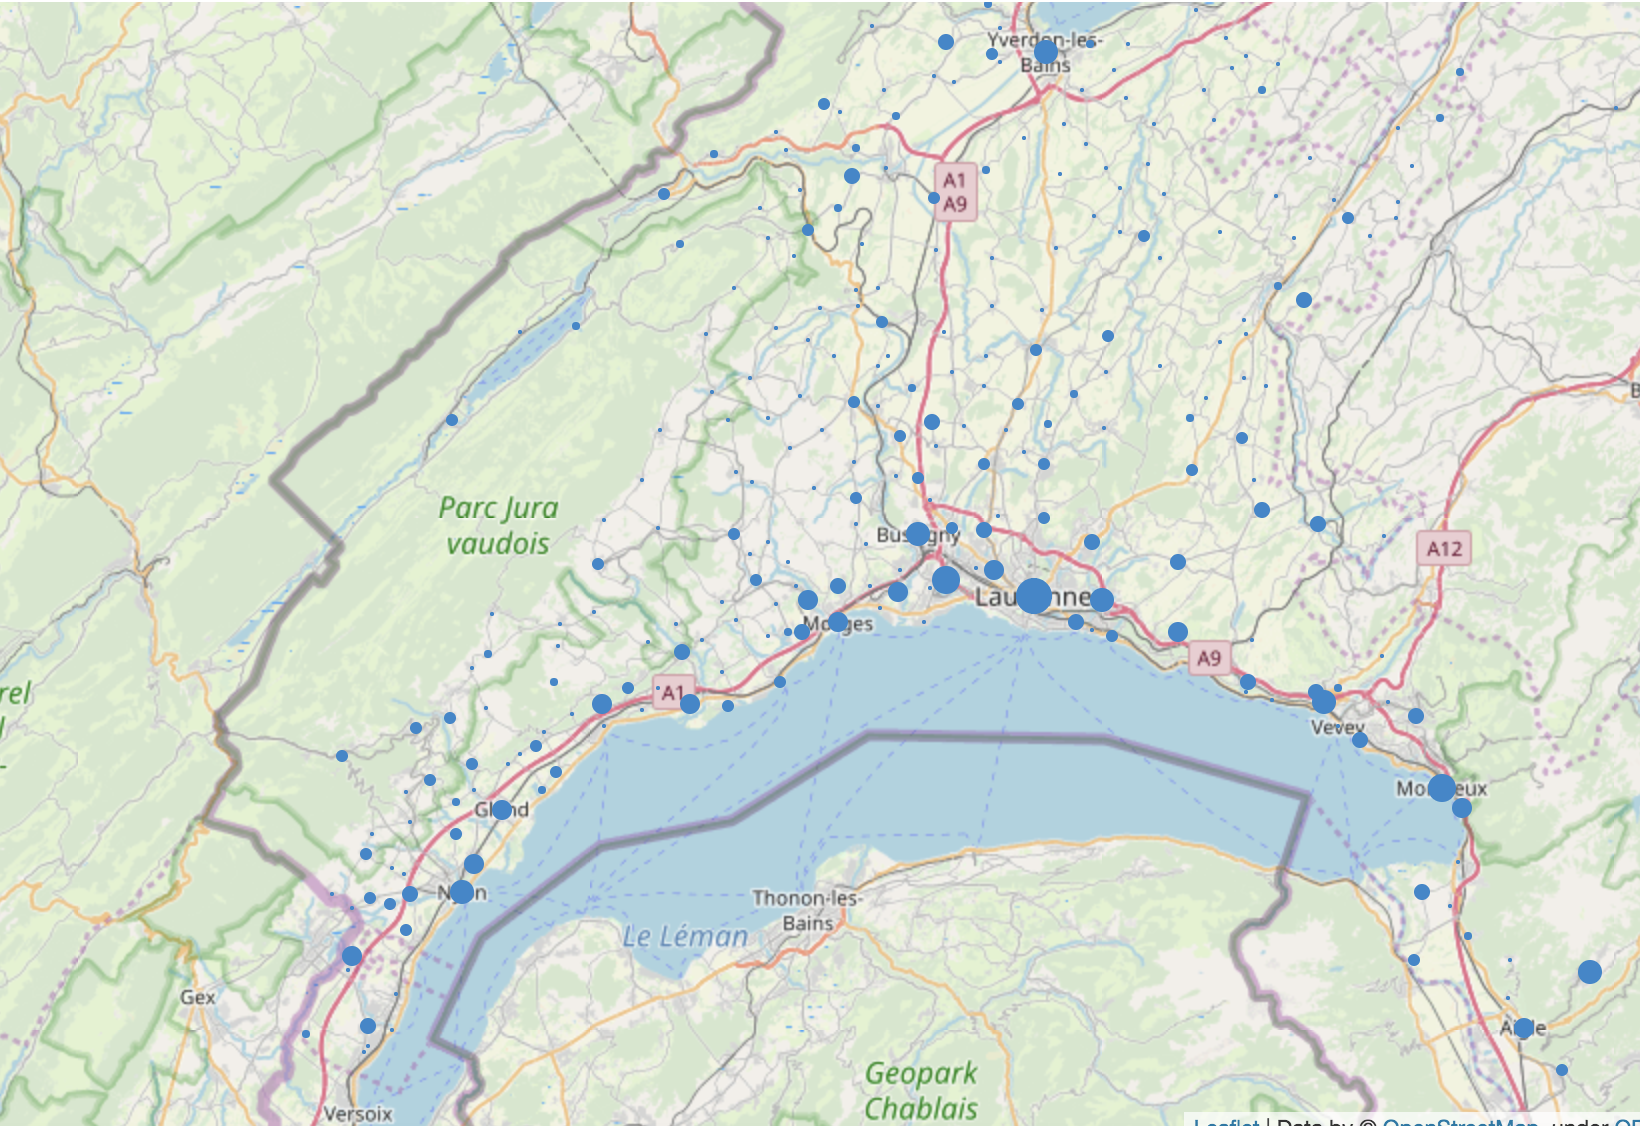
\includegraphics[width=\textwidth]{Figures/Fig3}
\caption{\label{fig3} Map representing each commune as a blue dot, with the radius being proportional to the logarithm of the total number of restaurants obtained for the commune.}
\end{center}
\end{figure}

\subsection{Restaurant statistics}

\begin{figure}
\begin{center}
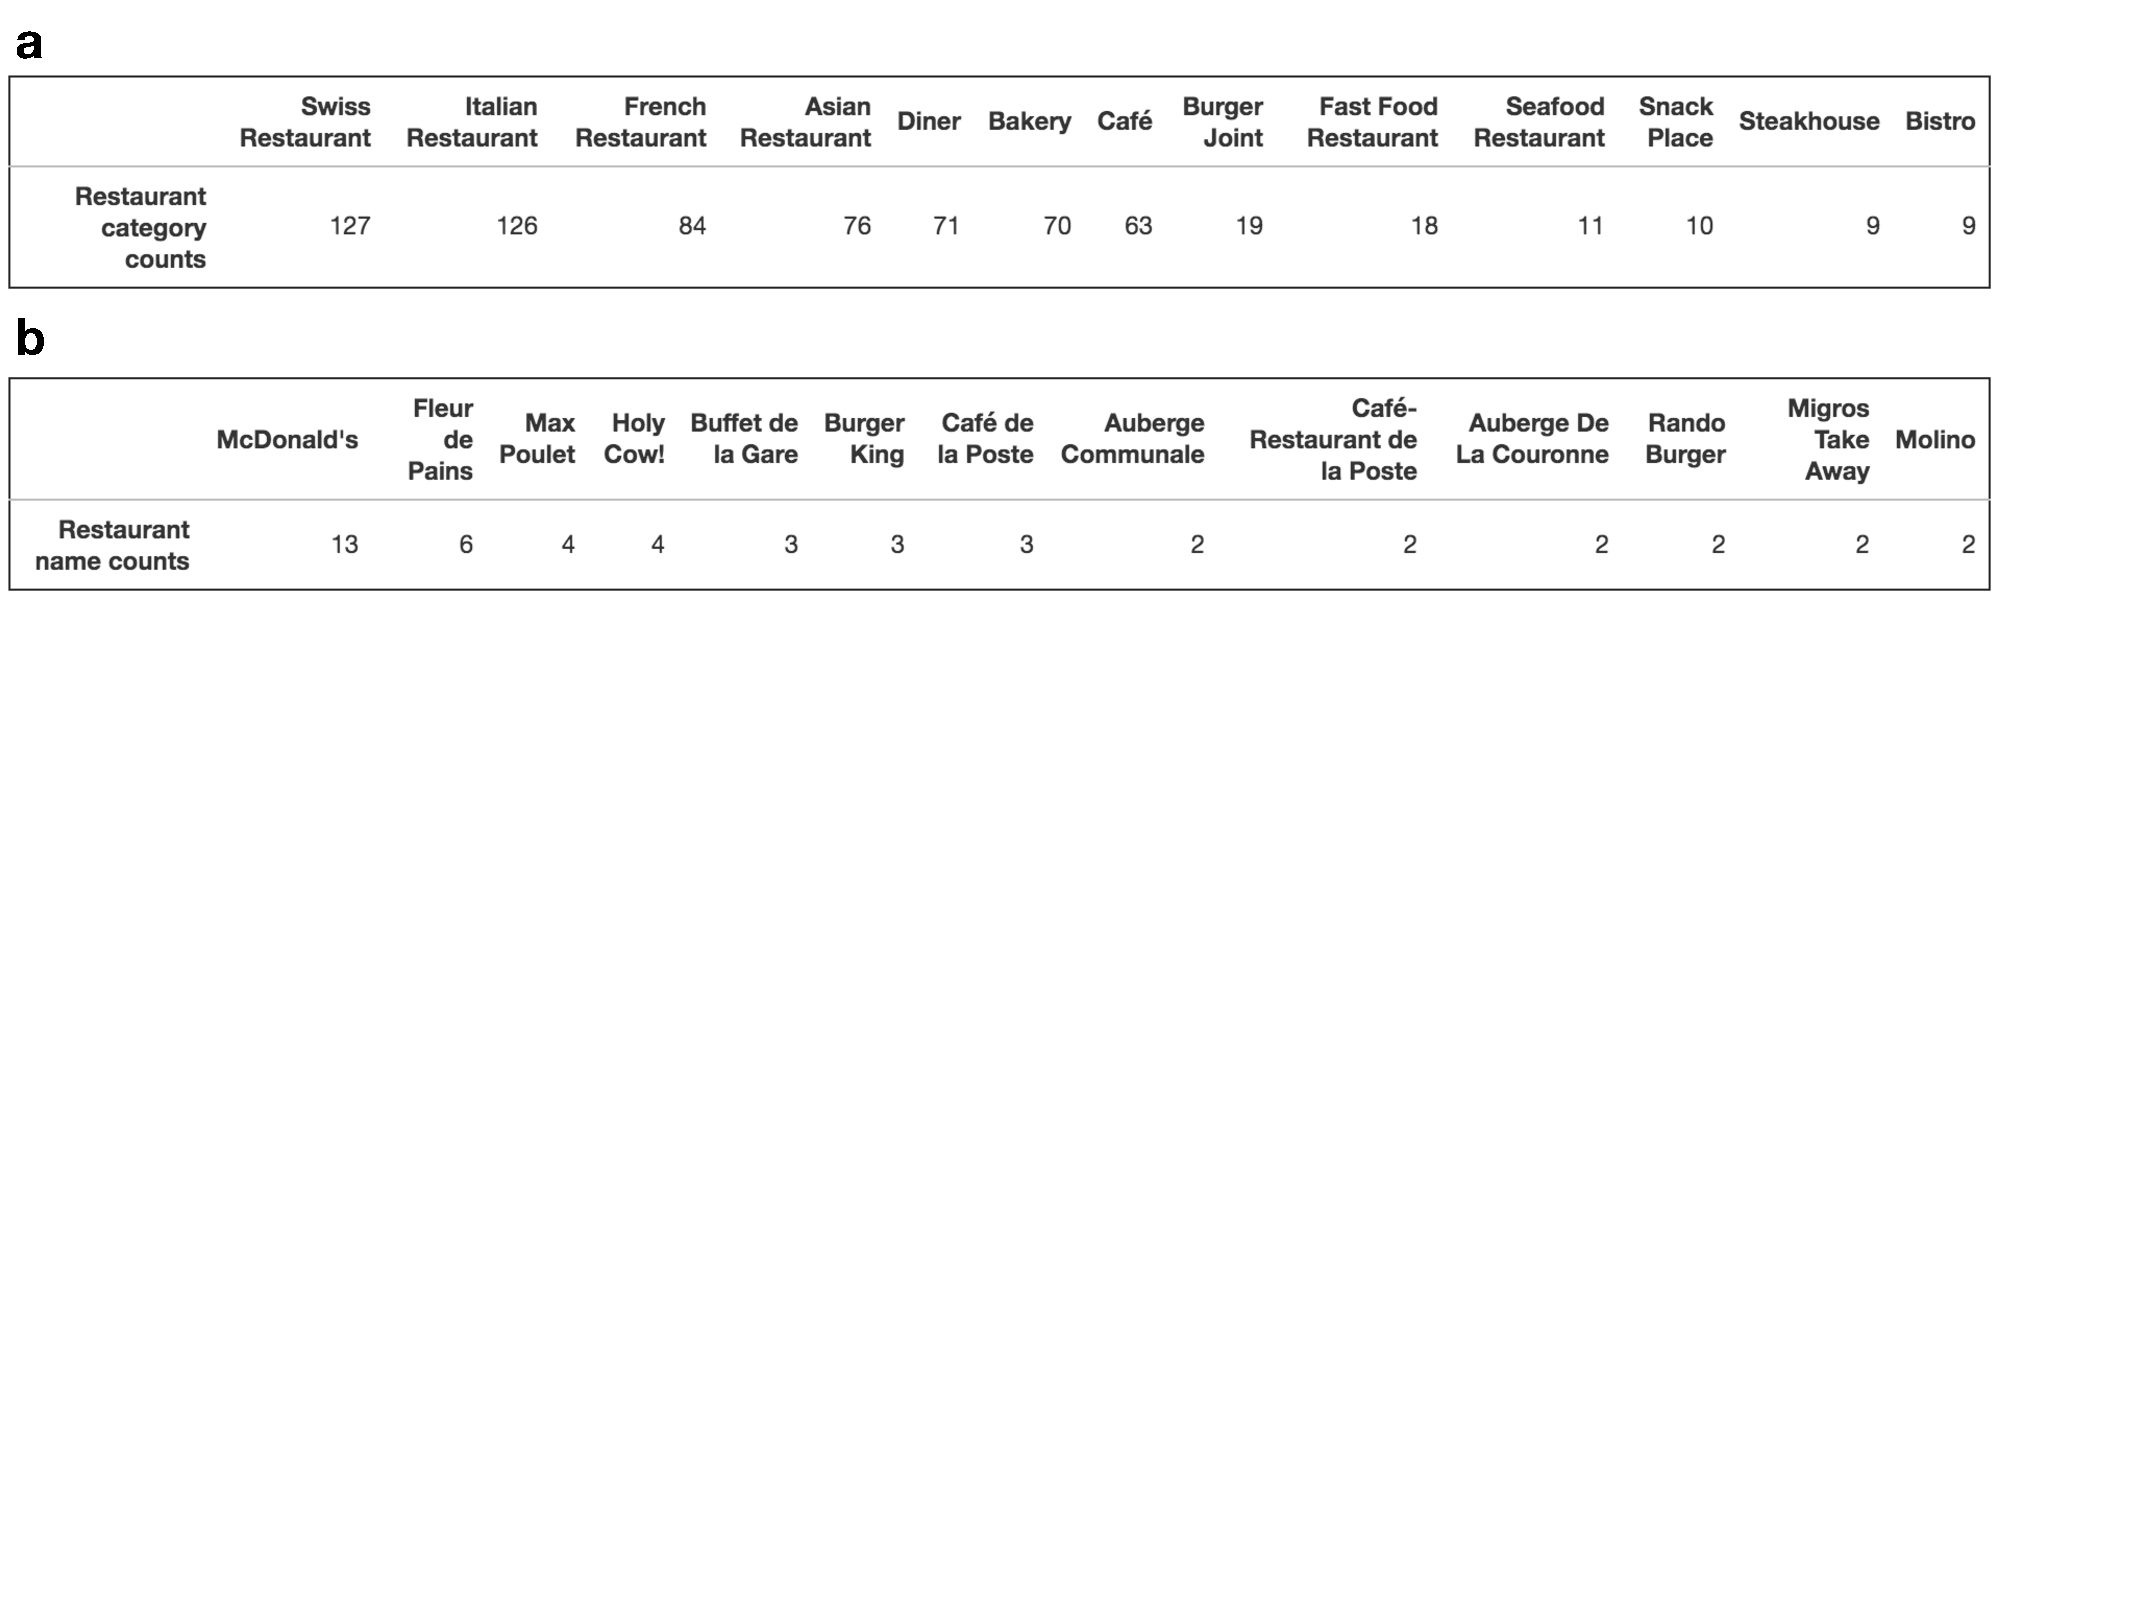
\includegraphics[width=\textwidth]{Figures/Fig4}
\caption{\label{fig4} (a) Restaurant categories, and (b) restaurant names, with the highest count among the 819 restaurant items.}
\end{center}
\end{figure}

The restaurants categories with the highest counts are represented in Fig.~\ref{fig4}(a). We see that, among the 819 restaurants, almost a third were either Swiss or Italian. Fig.~\ref{fig4}(b) shows the names with the highest frequency, which is by far dominated by the McDonald's chain.

\subsection{District properties and statistics}

\begin{figure}
\begin{center}
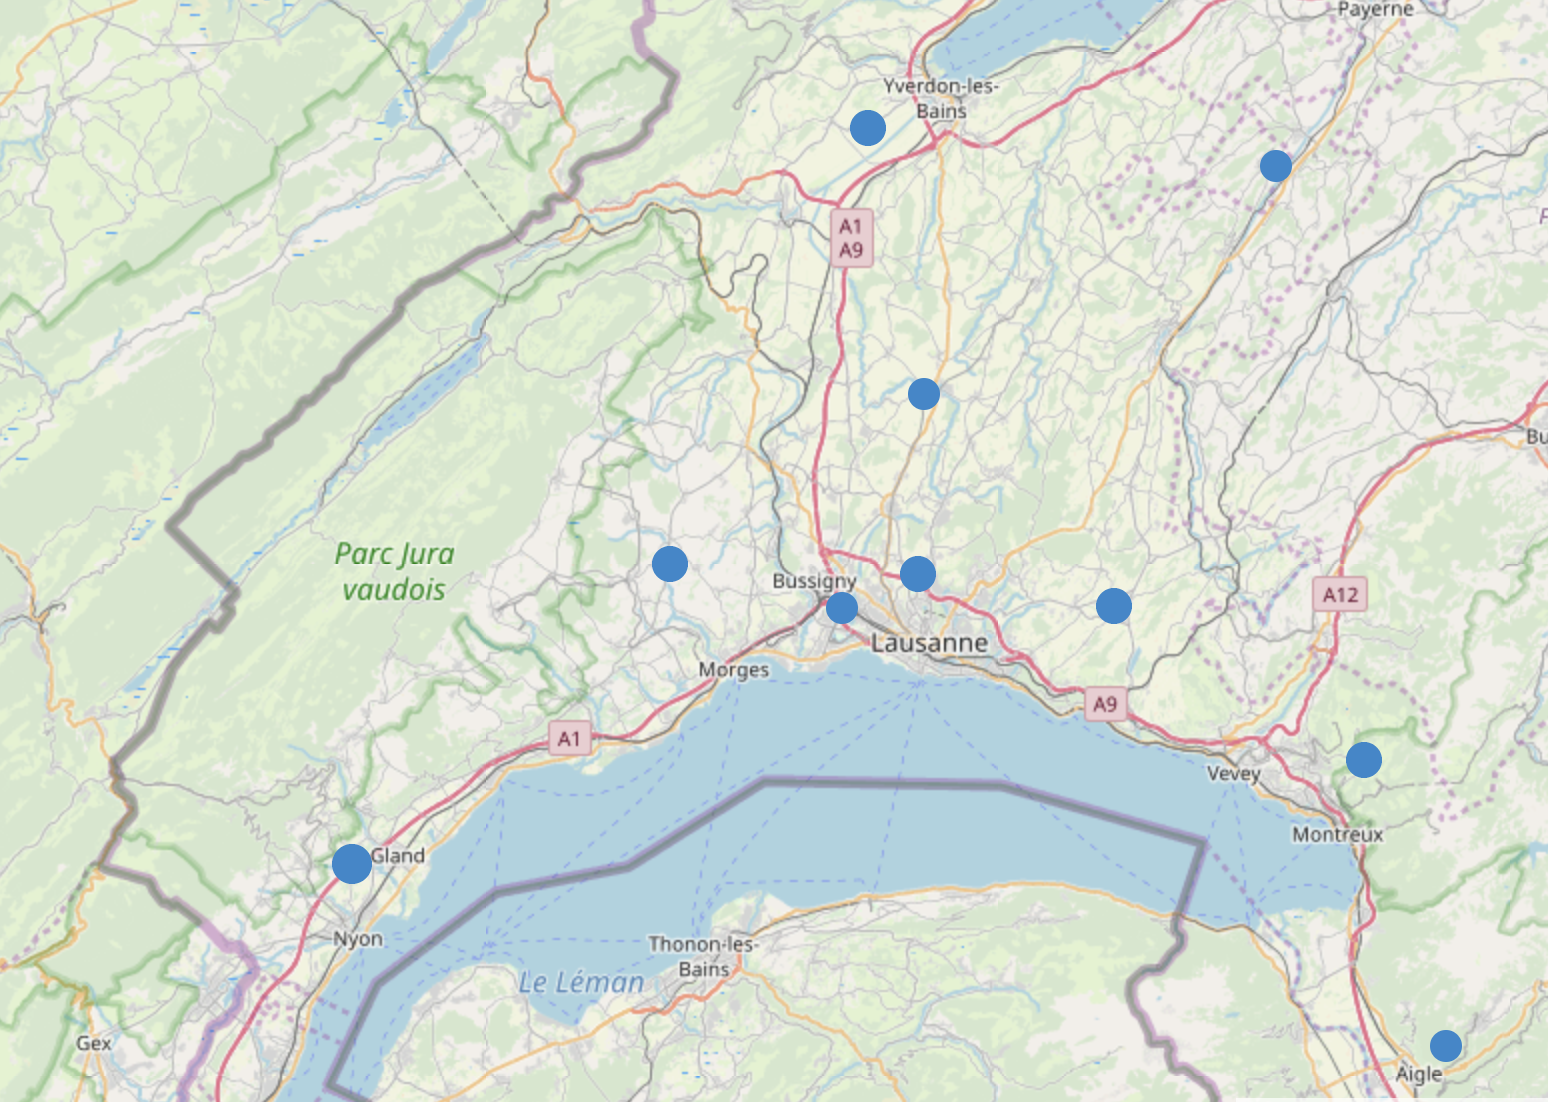
\includegraphics[width=\textwidth]{Figures/Fig5}
\caption{\label{fig5} Map representing each district as a blue dot, with the radius being proportional to the logarithm of the total number of restaurants obtained for the communes in the district.}
\end{center}
\end{figure}

Since it can be hard to infer properties on the communes from the statistics of their restaurants, as the number of restaurants can be very low (e.g. of order $1$ for small communes), we agglomerate the communes into their respective district. There are ten districts in the canton of Vaud, as represented in Fig.~\ref{fig5}.

\begin{figure}
\begin{center}
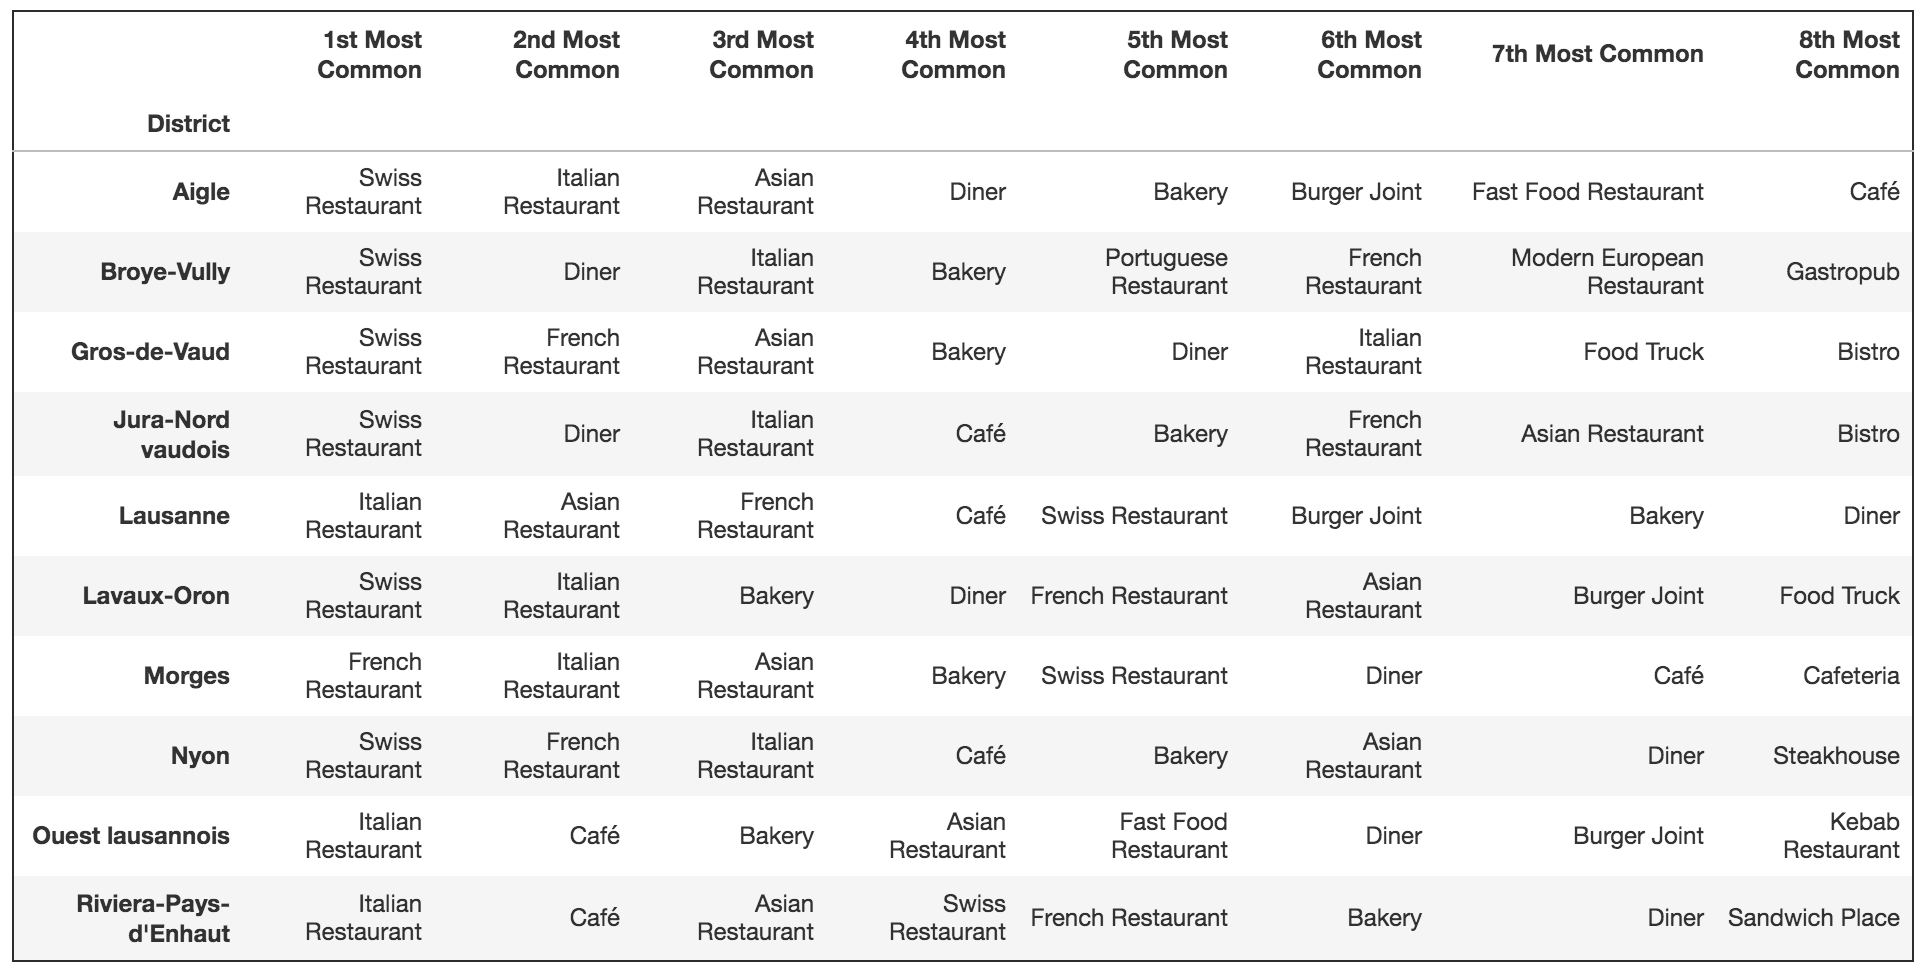
\includegraphics[width=\textwidth]{Figures/Fig6}
\caption{\label{fig6} Most common restaurant categories for each district.}
\end{center}
\end{figure}

In Fig.~\ref{fig6} we represent the most frequent restaurant categories obtained for each district. It is already visible that some district have distinguishable features, e.g. in their most common restaurant categories.


\subsection{Clustering communes and districts}
As we will show and discuss in the following Section, we applied k-means clustering algorithms in order to study how different categories of restaurants are distributed throughout the canton. In Sec.~\ref{sec:resultsa} we show how districts cluster together. For the clustering algorithm we convert each restaurant category to a dummy variable representing the proportion of restaurants belonging to that category, for each district. We also apply a hierarchical clustering algorithm, and study whether the clusters obtained are compatible between the two algorithms. 

In Sec.~\ref{sec:resultsb}, we show how communes, rather than districts, form clusters. We use, again, the restaurant categories as dummy variables for the algorithm. We study the average properties of each cluster. Finally, in order to acquire insight on the cluster formation, we also apply a decision tree algorithm allowing to predict to which cluster each commune should be assigned, depending on the restaurants obtained in that commune. 

\section{Results}\label{sec:results}

\subsection{Clustering districts}
\label{sec:resultsa}

\subsubsection{K-means clustering: 2 clusters}

\begin{figure}
\begin{center}
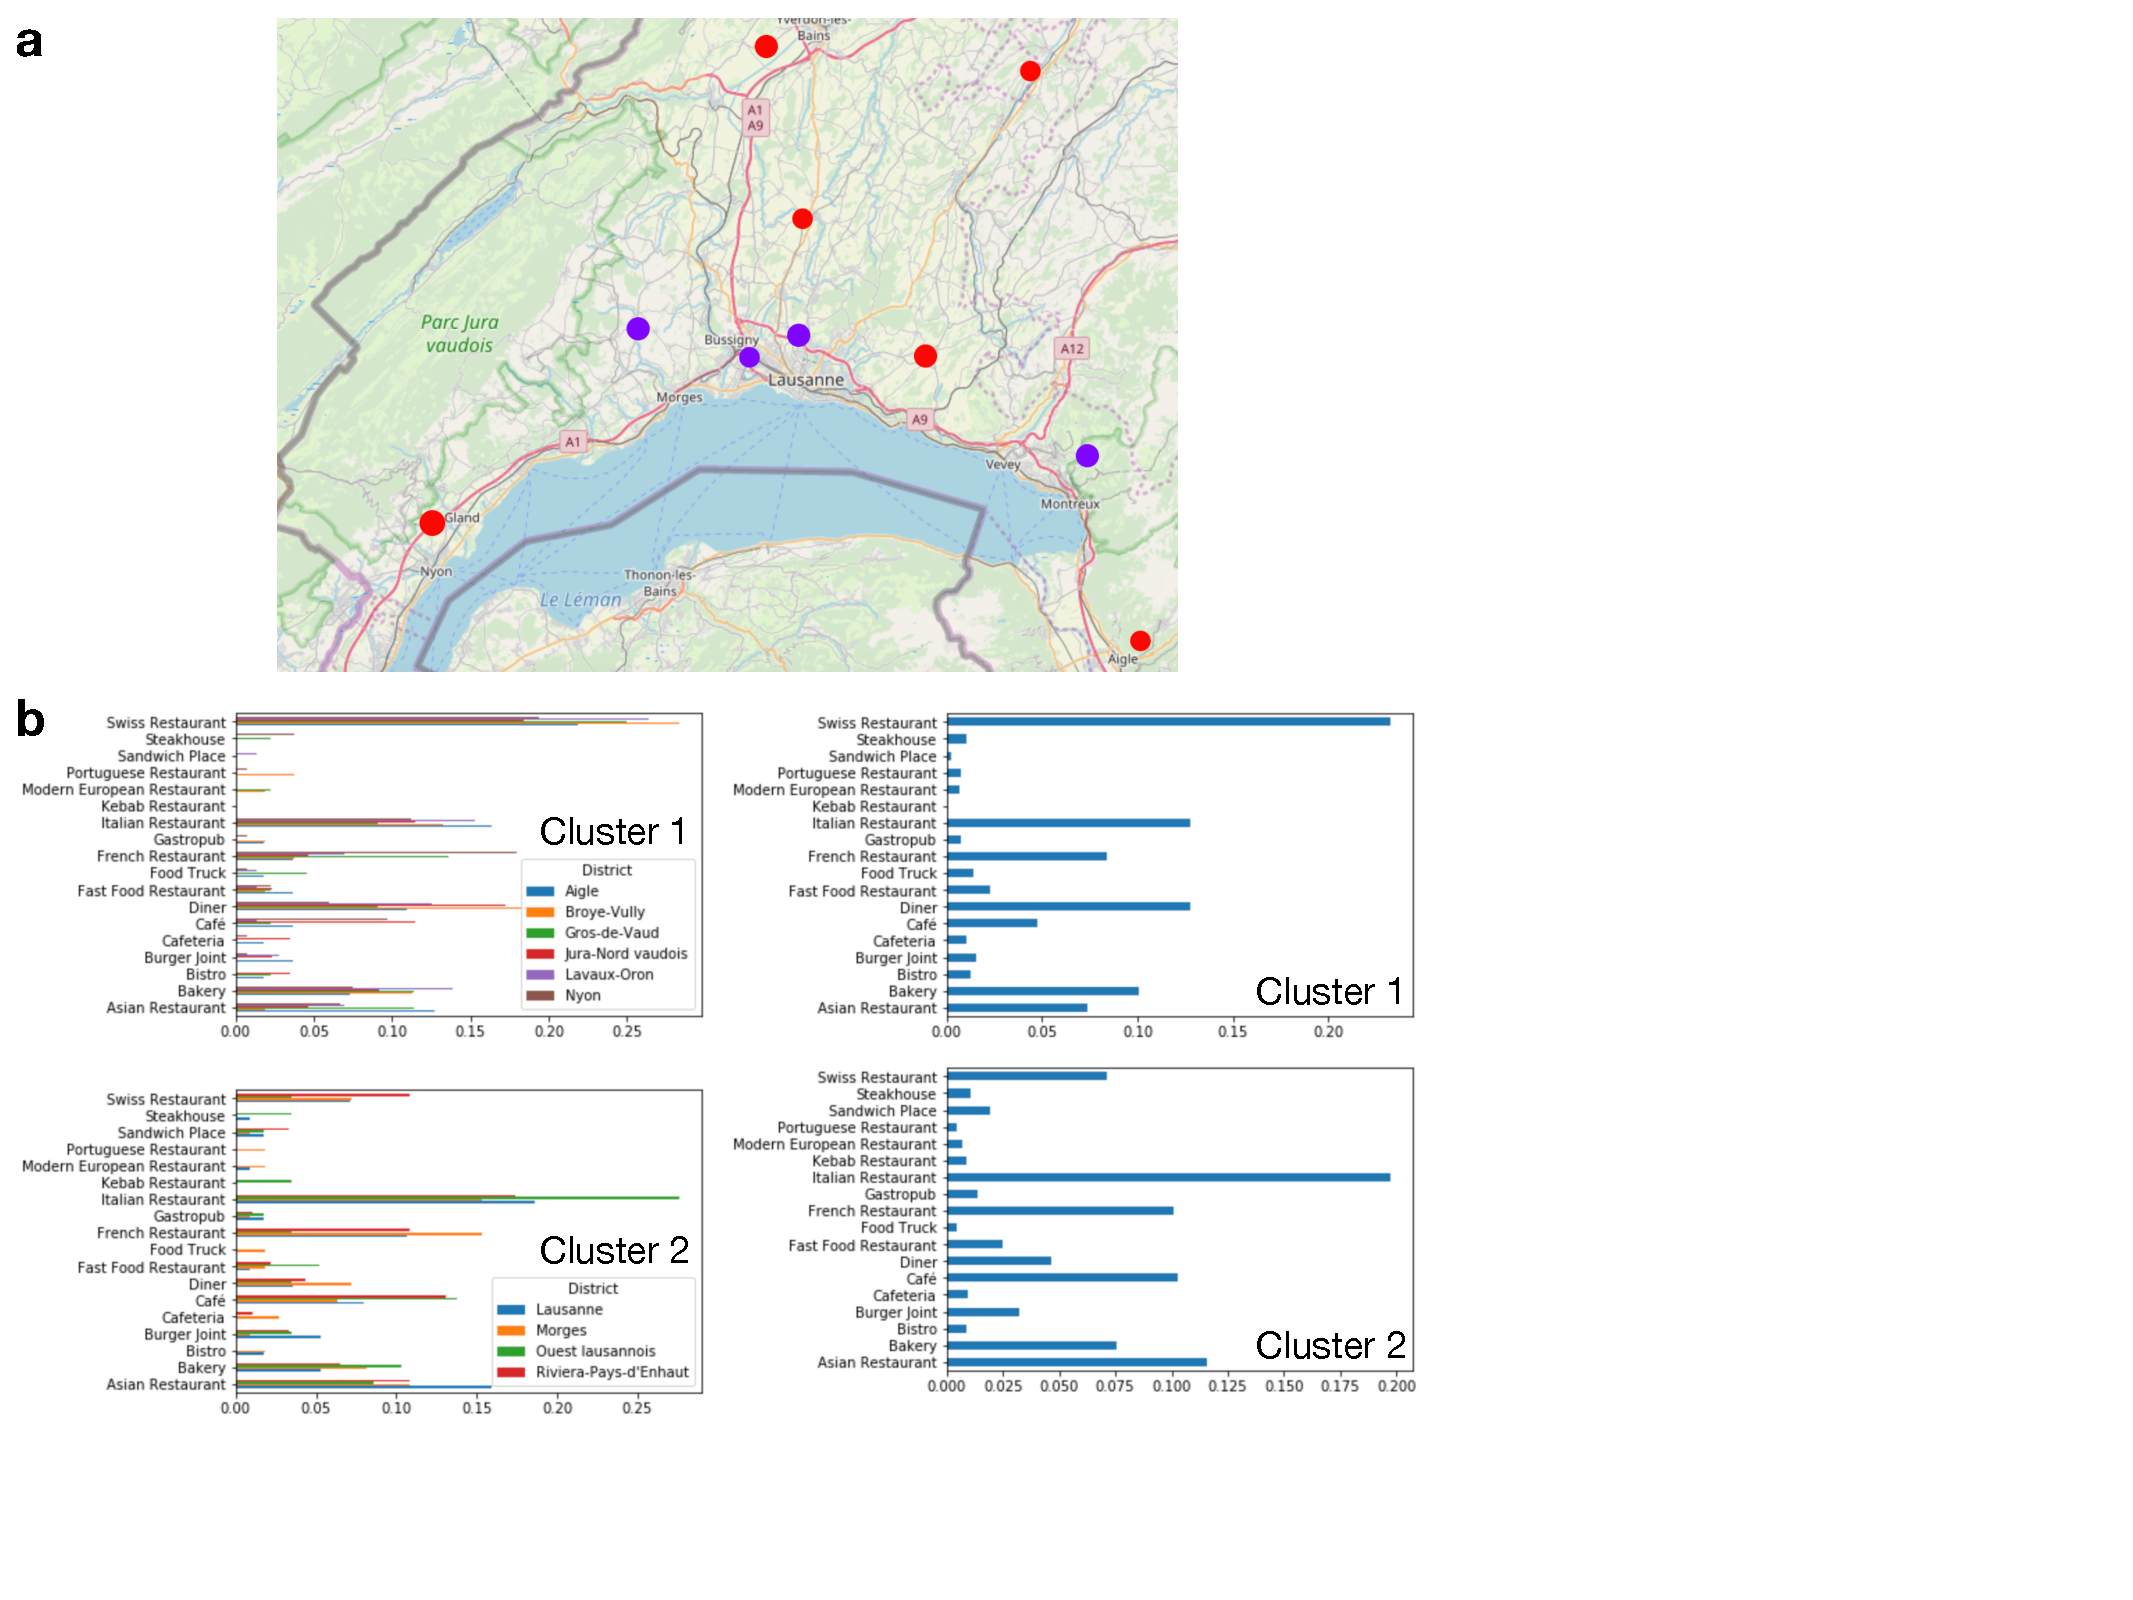
\includegraphics[width=\textwidth]{Figures/Fig7}
\caption{\label{fig7} \emph{K-means clustering on districts with 2 clusters.} (a)~Map representing the two clusters, with districts in cluster 1 shown in red dots and cluster 2 in violet dots. (b) Proportion of restaurant categories in each district (left), and averaged over the districts in each cluster (right).}
\end{center}
\end{figure}

In Fig.~\ref{fig7} we show the results when applying a k-means clustering algorithm with 2 clusters on the districts. The typical restaurant categories clearly differ for the two clusters, as represented in Fig.~\ref{fig7}(b). For districts in cluster $1$, we observe a predominance of Swiss restaurants, followed by Italian restaurants and diners. In Fig.~\ref{fig7}(a), we see that these rural districts are mostly located outside the larger population areas, and are typically constituted of countryside areas. On the other hand, urban districts, located near the L\'eman lake and containing larger population areas, are found in cluster $2$, where Italian restaurants dominate, followed by Asian restaurants, French restaurants, and caf\'es. 

\subsubsection{K-means clustering: 3 clusters}

\begin{figure}
\begin{center}
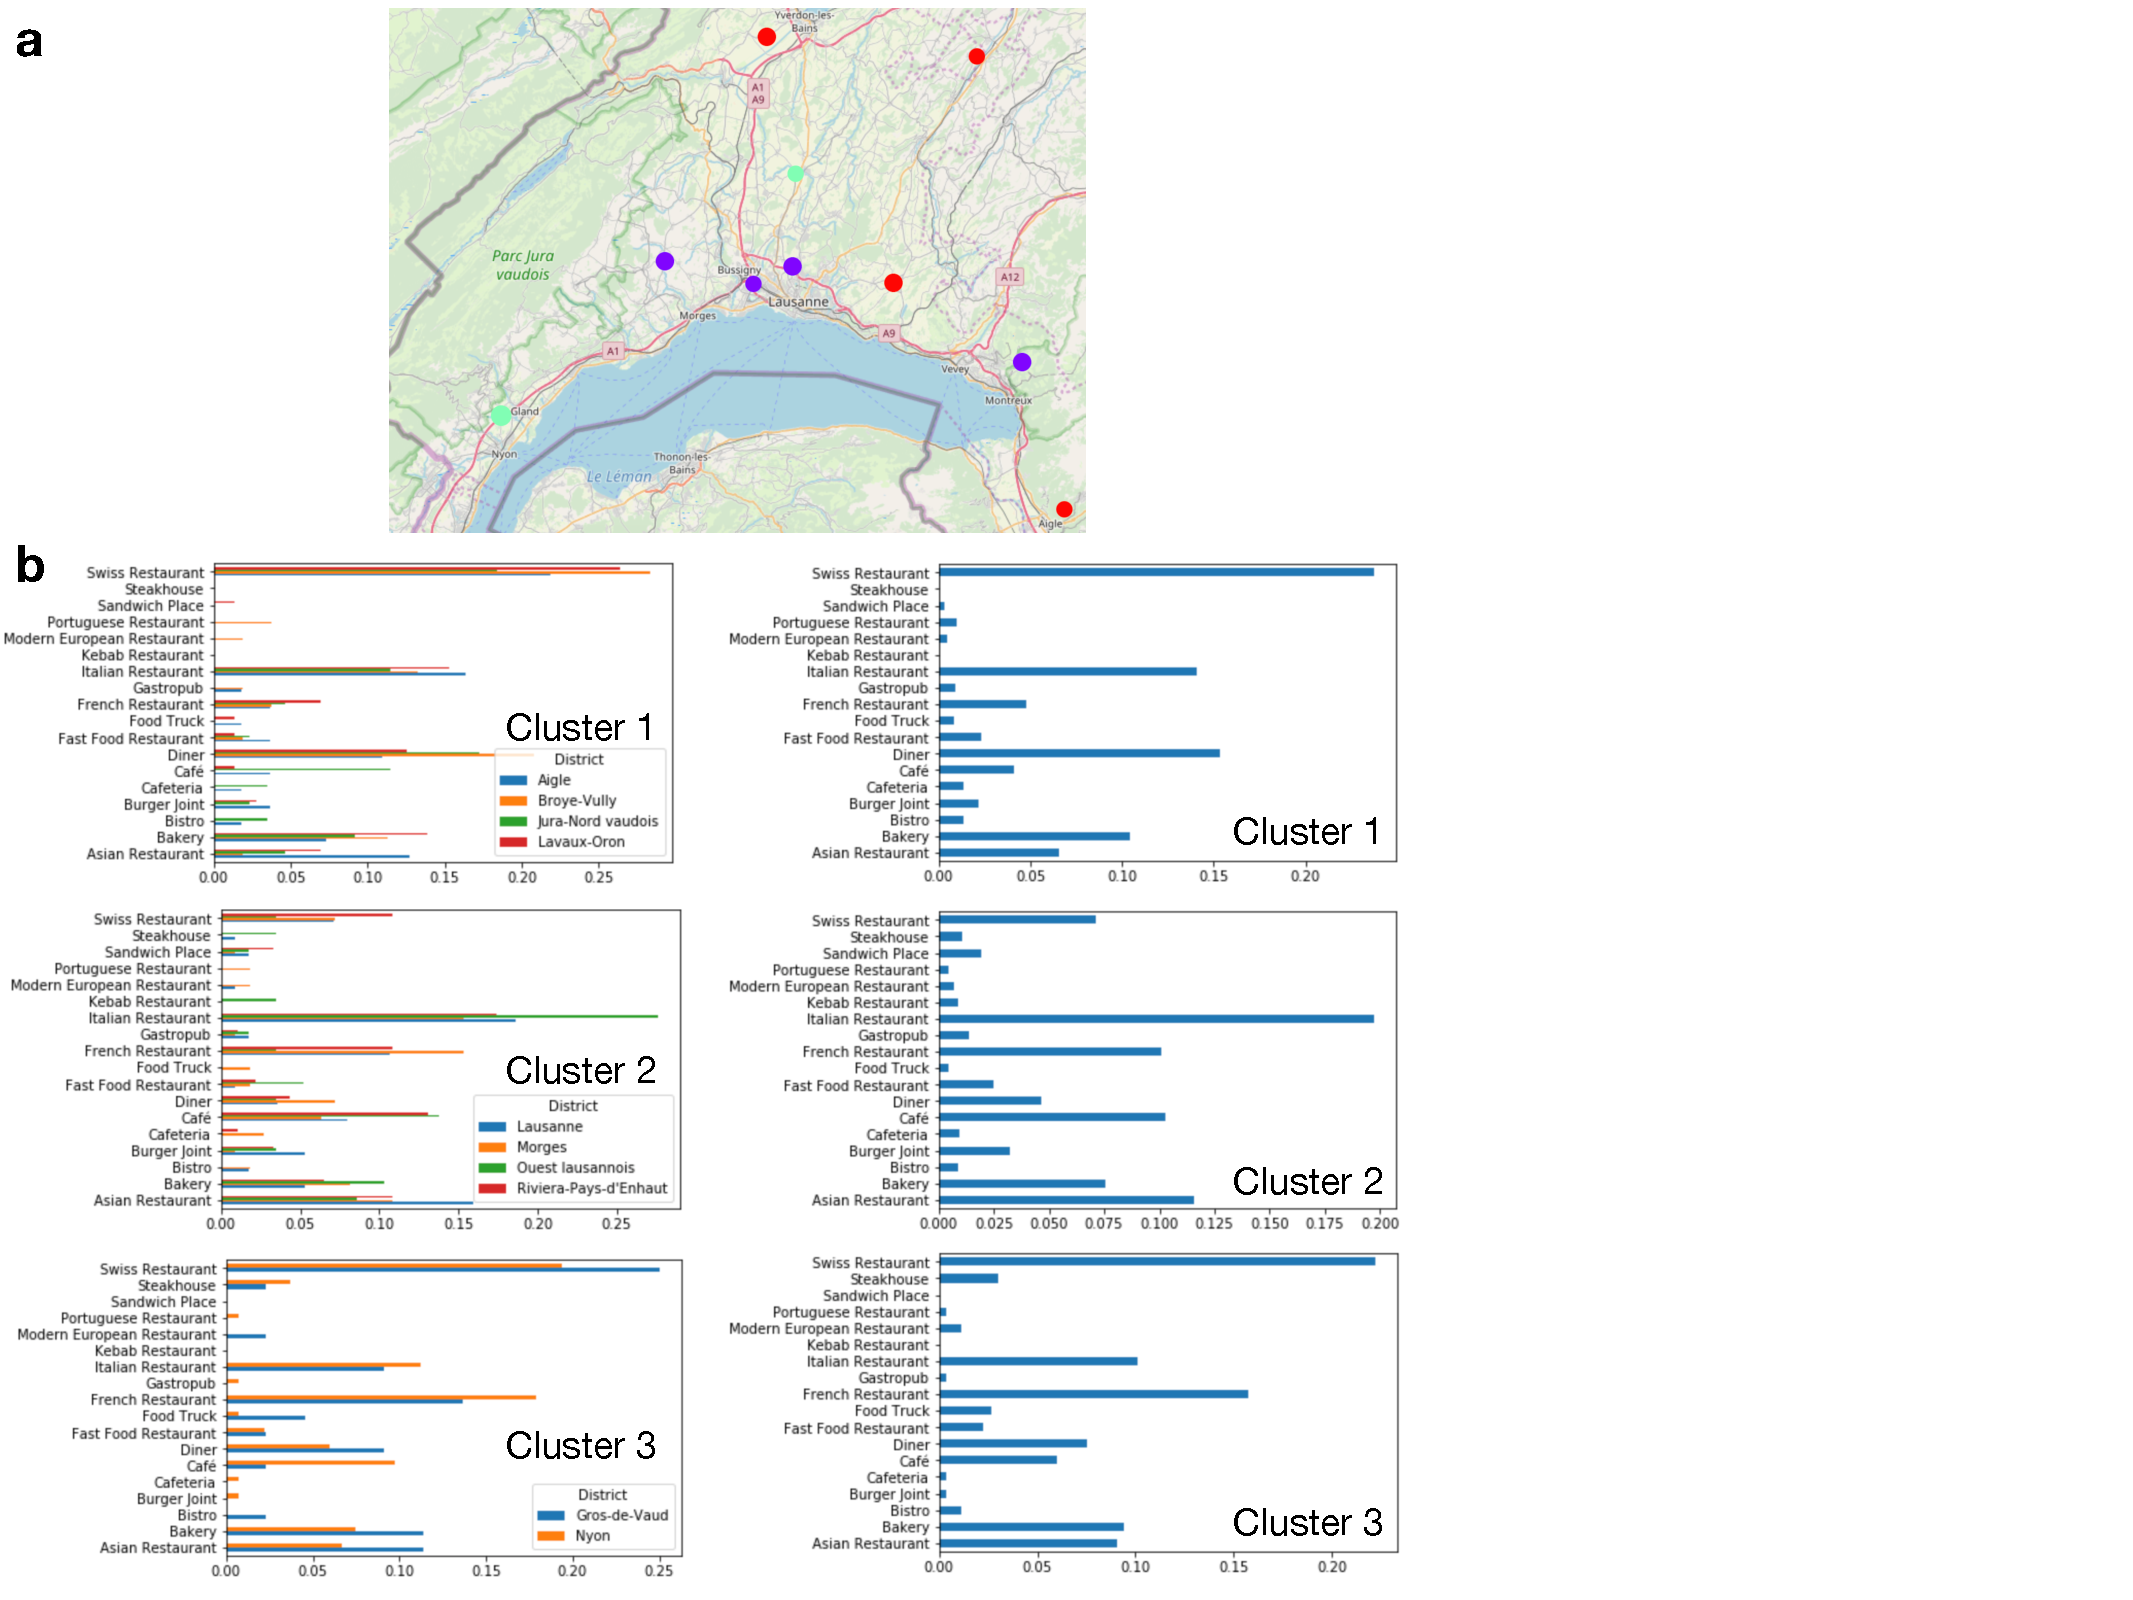
\includegraphics[width=\textwidth]{Figures/Fig8}
\caption{\label{fig8} \emph{K-means clustering on districts with 3 clusters.} (a)~Map representing the two clusters, with districts in cluster 1 shown in red dots, cluster 2 in violet dots, and cluster 3 in green dots. (b) Proportion of restaurant categories in each district (left), and averaged over the districts in each cluster (right).}
\end{center}
\end{figure}

In Fig.~\ref{fig8} we show the results when applying the clustering algorithm with 3 clusters. We see that, from the 2-cluster situation of Fig.~\ref{fig7}, cluster 1 has now been split into cluster 1 and 3. The typical features of the districts in cluster 3 can be interpreted as a mixture of that of the other two clusters, as seen in Fig.~\ref{fig8}(b).  


\subsubsection{Hierarchical clustering}

In Fig.~\ref{fig9} we show the results for the clusters obtained when applying an agglomerative clustering algorithm. Notably, both algorithms reproduce the results of the 2-cluster k-means algorithm in Fig.~\ref{fig7}.

\begin{figure}
\begin{center}
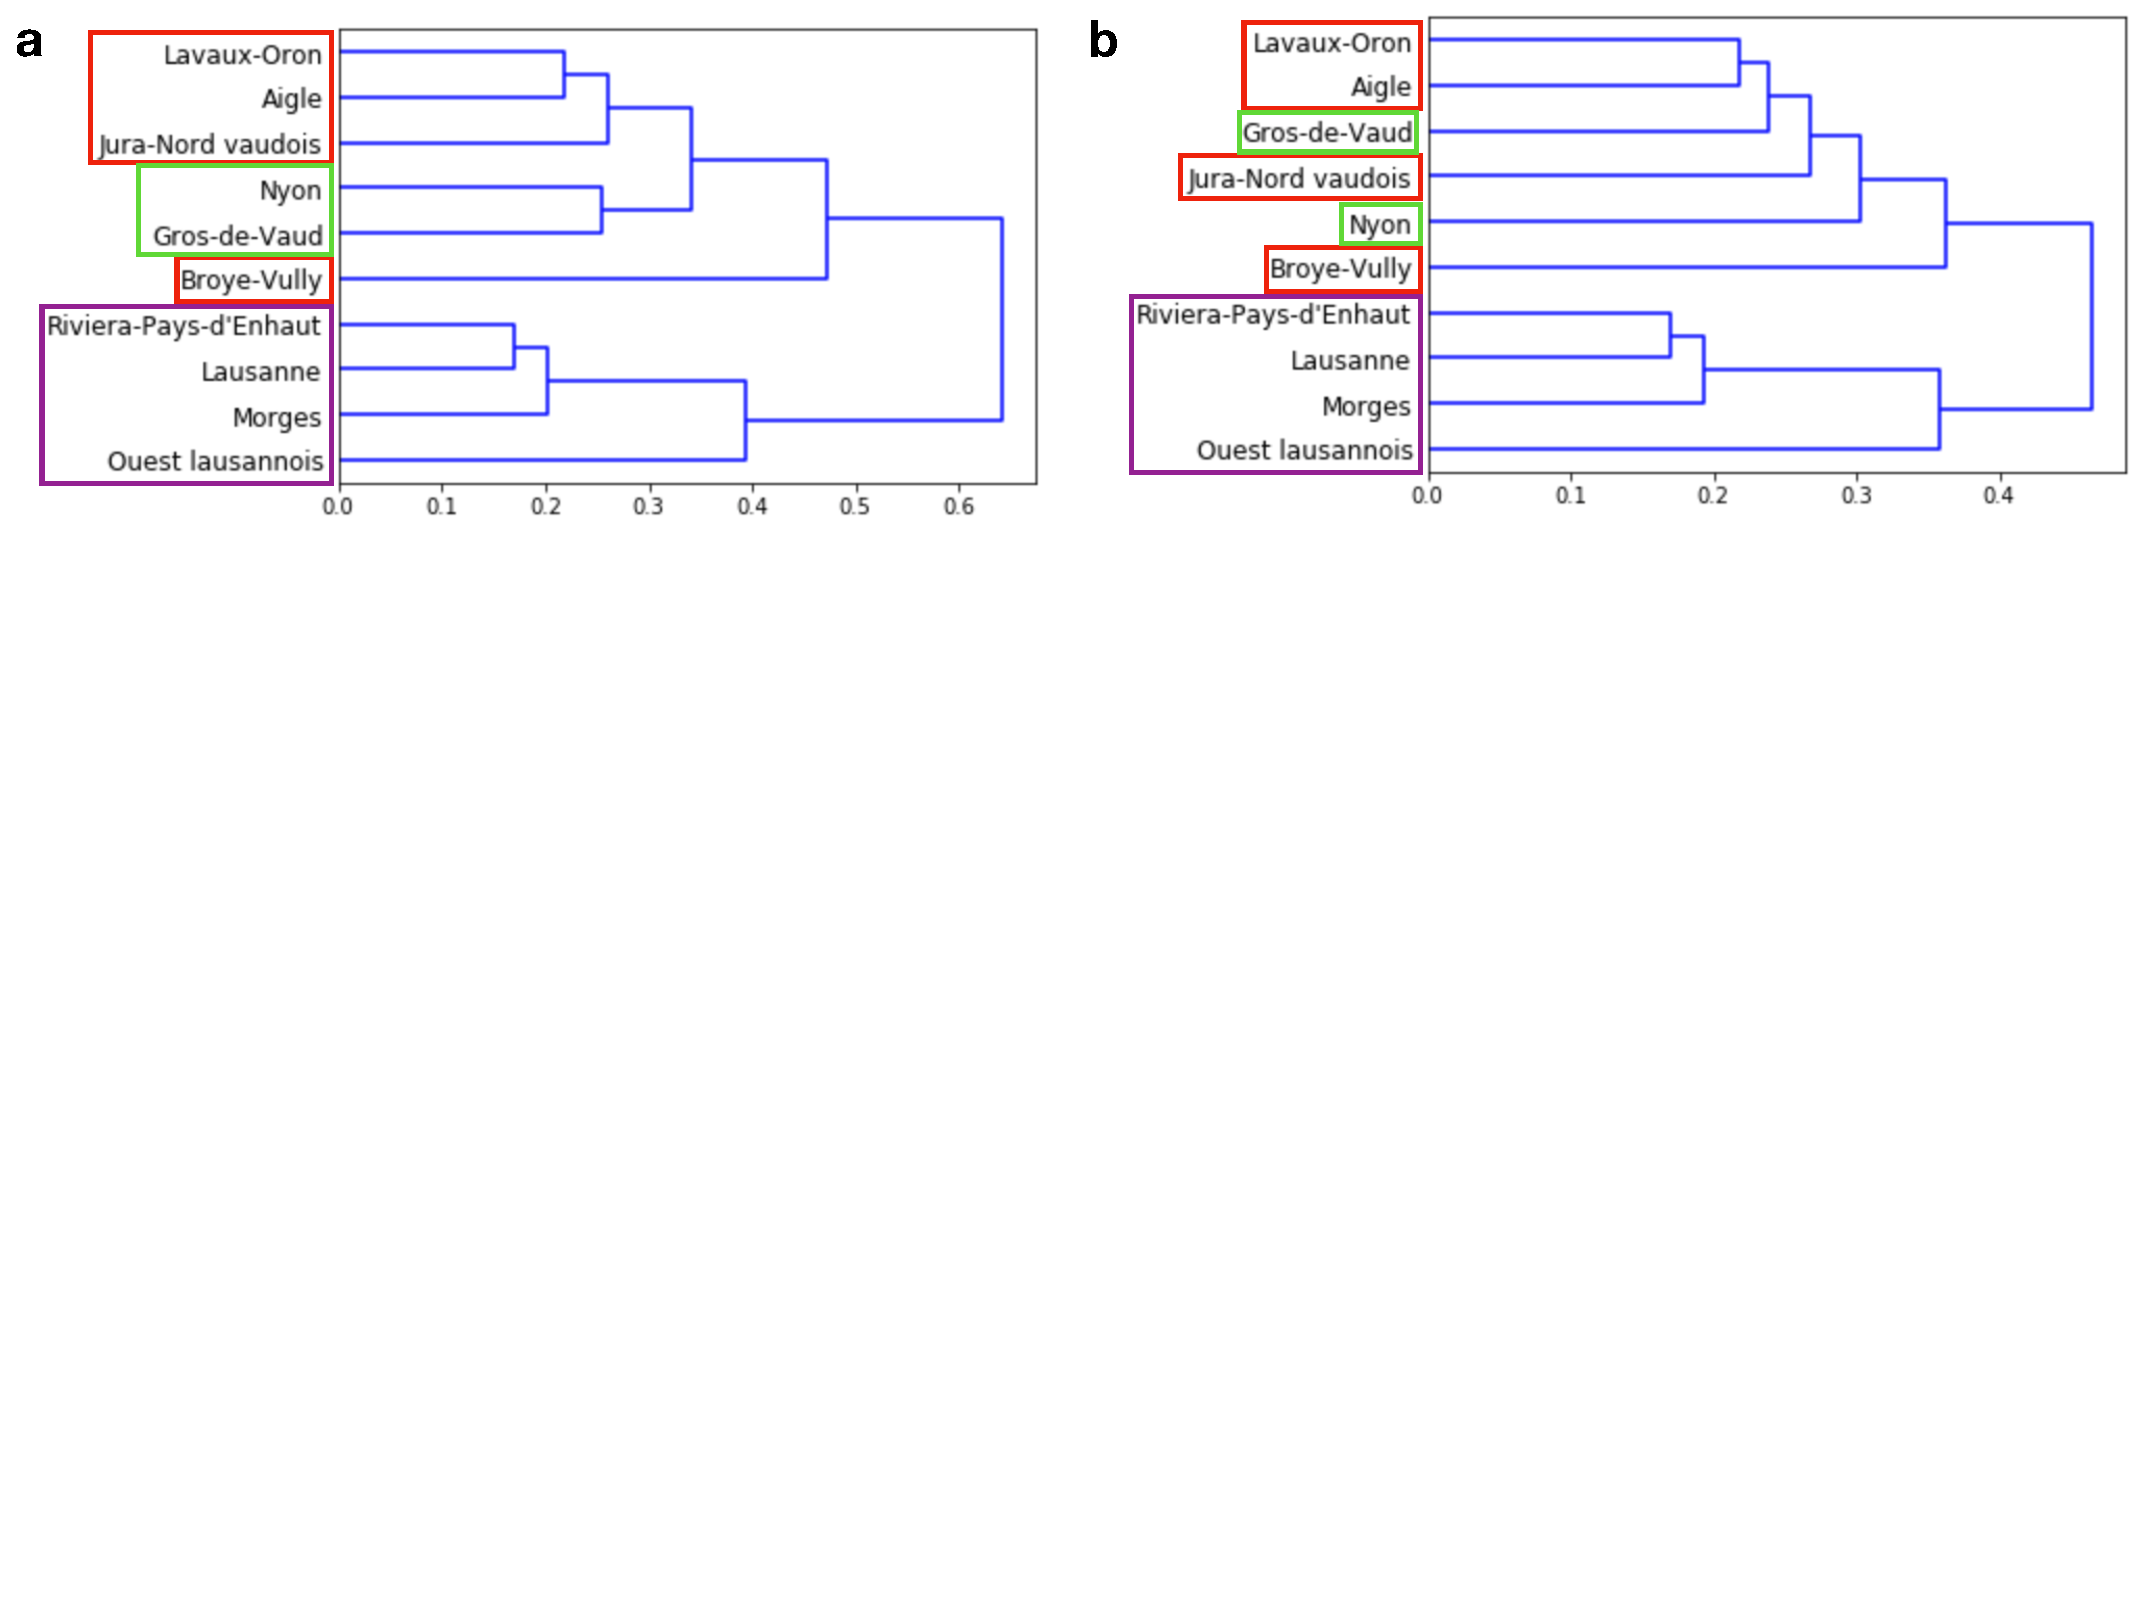
\includegraphics[width=\textwidth]{Figures/Fig9}
\caption{\label{fig9} \emph{Hierarchical clustering of districts.} Agglomerative clustering tree, using for the distance (a)~complete distance, and (b)~average distance.}
\end{center}
\end{figure}

\subsection{Clustering communes}
\label{sec:resultsb}

In order to cluster communes, rather than districts, we perform a similar k-means clustering algorithm, and vary the number of clusters. We found that the data was best clustered using four clusters, as a lower or higher number of clusters either led to disproportionate amounts of communes in one particular cluster, or to some clusters being almost empty. For four clusters, the properties are represented in Fig.~\ref{fig10}(a,b). We see that cluster 0 consists of communes with a relatively high population density, with on average a couple restaurants, and a predominance for Italian and French restaurants. They are represented in violet in the map of Fig.~\ref{fig10}(c). Cluster 1, represented in red on the map, constitutes most of the commune, with the highest average population density, and a diverse distribution of restaurant categories. Cluster 2, represented in blue on the map, is constituted of the smallest number of communes, with the lowest average population density and restaurant counts, and a large majority of diners.  
Finally, cluster 3, represented in green on the map, has a slightly higher population density and average restaurant obtained, with a predominance for Swiss restaurants. 

\begin{figure}
\begin{center}
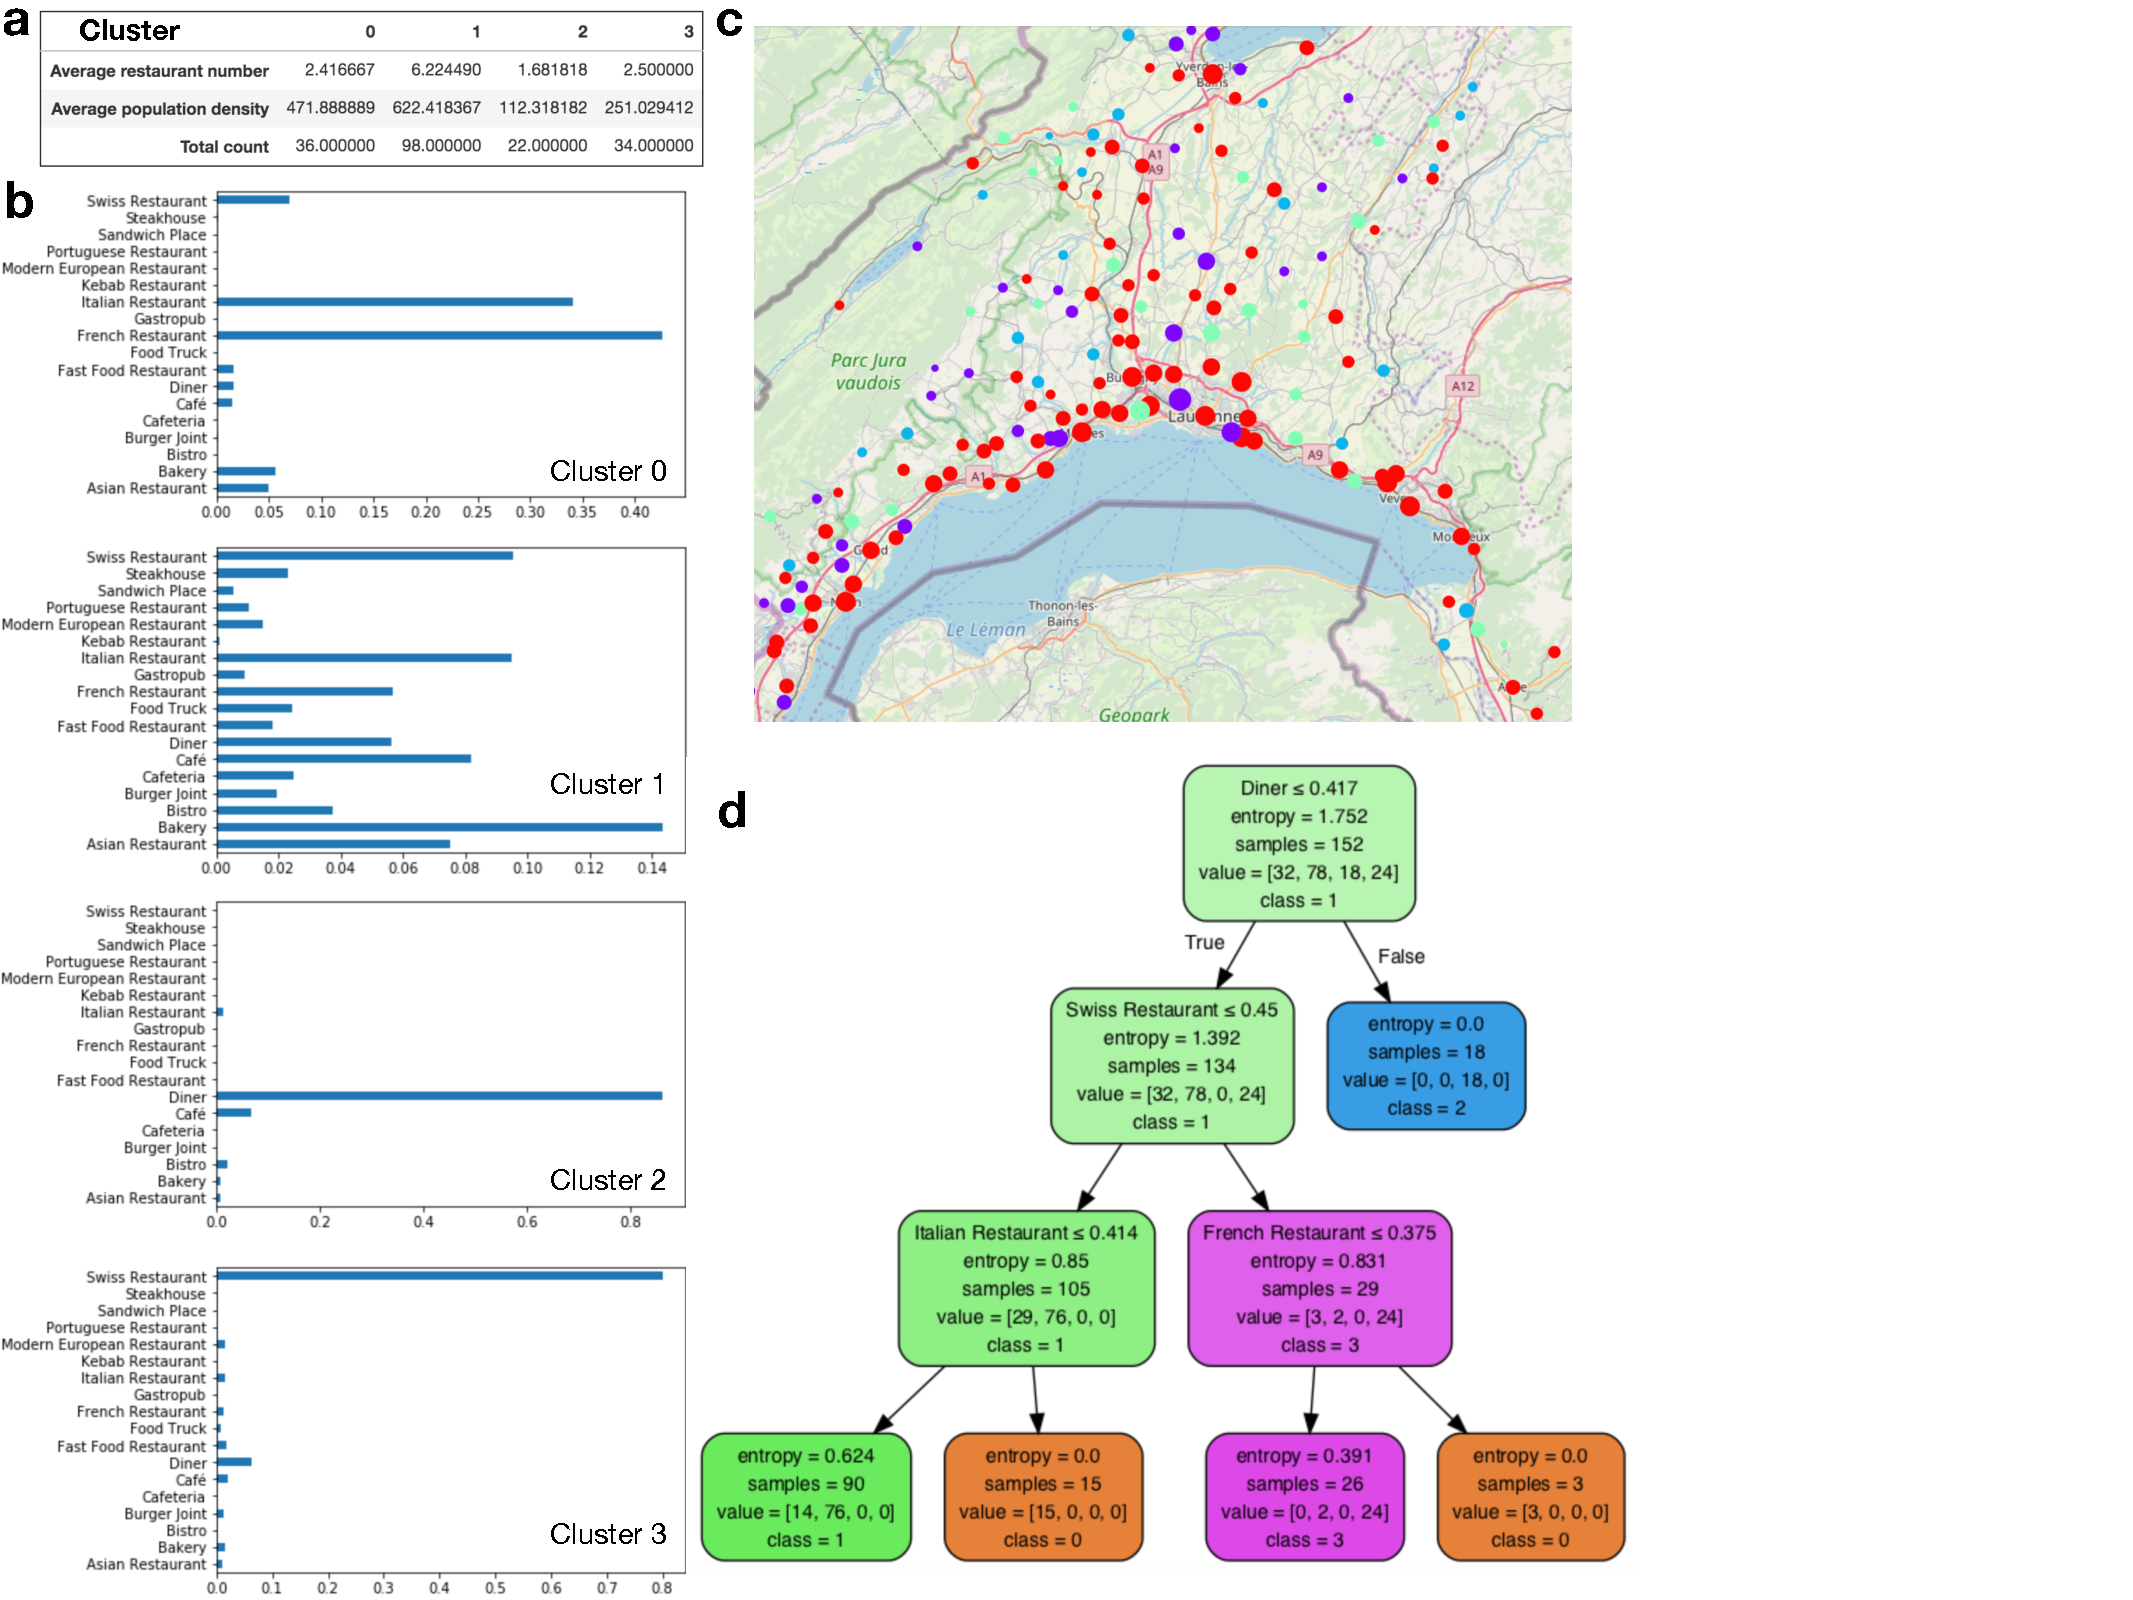
\includegraphics[width=\textwidth]{Figures/Fig10}
\caption{\label{fig10} \emph{Clustering communes into four clusters.} (a) Average number of restaurants, average population density, and total count for each cluster, labeled from 0 to 3. (b) Average proportion of restaurant categories in each cluster. (c) Representation of each commune, with communes in cluster 0 represented in violet, cluster 1 in red, cluster 2 in blue, and cluster 3 in green. (d) Decision tree obtained for classifying the communes in the four clusters, with an accuracy of 89\%.}
\end{center}
\end{figure}


Finally, in order to verify these relations between the typical restaurant categories and the clusters, we also applied a decision classification algorithm on the data set. We obtained a simple tree, with a depth of 3, which was tested on a fifth of the data with an accuracy of 89\%. The tree is represented in Fig.~\ref{fig10}(d), and reproduces the classification as described in the previous paragraph. We see that cluster 0 is typically assigned for communes with Italian or French restaurants, that cluster 2 is assigned for communes with a prevalence of diners, that cluster 3 is assigned for communes with Swiss restaurants, while cluster 1 represents communes with a diverse selection of restaurant categories. 

\section{Discussion}

The typical restaurant found in a given commune, or district, was found to depend strongly on the population density and the geographical location. In particular, the average distribution in Fig.~\ref{fig4} is not really representative of any area. Restaurants such as diners and Swiss restaurants are the typical types found in the countryside, i.e. in rural communes and districts with lower population density. The more urban areas have a much broader distribution of restaurant categories, including a prevalence for Italian, French or Asian cuisine. 


\section{Conclusion}

The study conducted here focussed only on the canton of Vaud. The cultural background of Switzerland is however quite diverse, and it would be interesting to extend the study to other regions. In particular, Switzerland also has a german-speaking part and an italian-speaking part; it would be interesting, and informative, to perform the same study on such regions, and observe wether similar results are obtained, or which regions have a larger diversity of restaurant categories.

\end{document}